%%This is a very basic article template.
%%There is just one section and two subsections.
\documentclass{article}

\usepackage{amsmath}
\usepackage{amscd}
\usepackage{amssymb}
\usepackage{amsfonts} 
\usepackage{amsthm}
\usepackage{amsfonts}
\usepackage{amsthm}

\usepackage{circuitikz}
\usepackage{pgf}
\usepackage{tikz}
\usetikzlibrary{arrows,snakes,backgrounds}
% \usetikz
\usepackage{subfig}

\usepackage{algpseudocode}
\usepackage{algorithm}

\usepackage[super]{nth}

% \usepackage{appendix}
% \usepackage{listings}
% \usepackage{color}

\usepackage{hyperref}
%\usepackage{url}

\usepackage{cleveref}
\usepackage{cancel}

\usepackage{aviolov_style}
\usepackage{local_style}


\newtheorem{thm}{Theorem}[section]
\newtheorem{lemma}{Theorem}[thm]
% \theoremstyle{definition}
\newtheorem{ex}{Example}[thm]
\newtheorem{defn}{Definition}[thm]

\usepackage{embedfile}
\embedfile{OptSpike.brief.tex}

\begin{document}


\title{Stochastic Optimal Control for spike control in single neurons
\\
\vskip3pt
brief - .tex attached (see attachmets in acrobat)
}
\author{Alexandre Iolov 
$<$\href{mailto:aiolo040@uottawa.ca}
		{aiolo040 at uottawa dot ca}$>$}

\date{\today}

\maketitle

\abstract{We pose an optimal control problem to precisely specify the spike
timing in a noisy leaky-integrate and fire model of a neuron. The optimal
control problem is solved using Dynamic Programming if we have access to the
voltage (closed-loop control) and using a Maximum Principle for the transition
density if we only have access to the spike timings (open loop control)}

\section{A Stochastic Optimal Control for Spike Timings Control}
Assume your neuron can be represented by a leaky-integrate and fire model
\begin{equation}
\begin{gathered} 
dX_t = \left(\a(t) - \frac{X_t}{\tc} \right) \intd{t} + \b \intd{W_t},
\\
X(0) = .0,
\\
X(\ts) = \xth \implies  
\begin{cases}
X(\ts^+) = .0 &  
\end{cases}
\end{gathered}
\label{eq:X_evolution_uo}
\end{equation}
We look for the control, $\a(t)$, which will minimize the squared distance
between the realized spike time, $\ts$ and a desired, pre-determined time $\T$.
\begin{equation}
\a(t) = \argmin_{\a(t)} \{\, \Exp[(\ts- \T)^2] \,\}
\label{eq:OC_LS_variance}   
\end{equation}
where expectation is taken with respect to the trajectories of $X_t$.

We consider two scenarios, one, {\sl closed loop control}, in which the
value of $X_t$ at $t$ is known and can be used in determining the control and
,two, {\sl open loop control} in which only the times of spikes is known. In
closed-loop scenario, we might better write the control as
$$\a = \a(x,t)$$ to indicate its dependence on $X_t$. In the open-loop scenario,
we would instead write $$\a = \a(t)$$ to indicate that we will always do the
same thing regardless of the (unknown) behaviour of $X_t$. 

For the closed-loop scenario we will use {\sl Dynamic Programing},
\cite{Fleming1975}, while for the open-loop scenario we will use a form
of the {\sl Maximum Principle} for transition densities, \cite{Ahmed1981}.

\section{Closed-Loop Solution - Dynamic Programing}
Given $t, X_t = x$, let $\t$ be the (unknown) remaining time to spike. For
example, given $t=0, X=.0$, $\t = \ts$, the entire duration of the inter-spike interval.
Starting from a general $t, x$, our remaining-cost objective, $J[\a; x,t]$,
will be:
\begin{equation}
J[\a, x,t]  = \Big\{ \,
\Exp\left[
\e \int_t^\ts  \a^2 \intd{s}
+
(\ts - \T) \big)^2 |x,t
\right] \, \Big\}
\label{eq:OC_LS_mean_objective}   
\end{equation}

Setup the Hamilton-Jacobi-Bellman (HJB) equation
\cite{Fleming1975} for this problem by first introducing the value function, $v(x,t)$ as: 
\begin{align}
v(x,t) =& \argmin_{\a(s \geq t)} \{J[\a, x,t] \}
\notag 
\\ 
=&
\argmin_{\a(s \geq t)} 
\Big\{ \,
\Exp\left[
\e \int_t^\ts  \a^2 \intd{s}
+
(\t - (\T-t) \big)^2 |x,t
\right] \, \Big\}
\label{eq:OC_LS_mean_value}   
\end{align}

The corresponding HJB PDE for $v$ is:
\begin{equation}
\di_t v(x,t) + \tfrac{\b^2}{2} \di_x^2 v + \min_{\a \in [\amin, \amax]}\big\{
\e \a^2 + (\a-\tfrac{x}{\tc}) \di_x v \big\} = 0
\label{eq:OC_LS_mean_HJB}
\end{equation}
and the optimal control is given by:
\begin{align}
\a(x,t)  =&\argmin_{\a \in [\amin, \amax]}\big\{
\e \a^2 + (\a-\tfrac{x}{\tc}) \di_x v \big\}
\notag 
\\
=& 
\min \left(\amax, \max\left(\amin, -\frac{\di_x v}{2\e}\right)
\label{eq:OC_LS_variance_energy_quadratic_control}
\end{align}
With this the HJB becomes
\begin{equation}
\di_t v(x,t) + \tfrac{\b^2}{2} \di_x^2 v + 
\e (\astar)^2 + (\astar-\tfrac{x}{\tc}) \di_x v 
= 0
\label{eq:OC_LS_mean_HJB_bounded_control}
\end{equation}
\Cref{eq:OC_LS_mean_HJB_bounded_control,eq:OC_LS_variance_energy_quadratic_control}
need to be solved simultaneously. 

Applying the right BCs and TCs for $v$ results in the fully specified HJB
equation
\begin{equation}
\begin{gathered}
\di_t v(x,t) + \tfrac{\b^2}{2} \di_x^2 v + 
\e \a^2 + (\a -\tfrac{x}{\tc}) \di_x v 
= 0
\\
\a (x,t) = \min \left(\amax, \max\left(\amin, -\frac{\di_x v}{2\e}\right)
\right)
\\
\begin{cases}
v(\xth,t) = (t-\T)^2  \quad & \textrm{upper BC}
\\
\di_x v(\xmin, t)  = .0  \quad &\textrm{lower BC}
\\
v(x,T)  = \Exp[\t^2|x, \amax]  \quad& \textrm{TC}
\end{cases}
\end{gathered}
\label{eq:OC_LS_HJB_full}
\end{equation} 
We are solving $v(x,t)$ over $[\xmin, \xth] \times [0,T]$.

A few words on the terminal conditions (TCs). $\Exp[\t^2|x, \amax]$ is the
expected time to spike (reach the threshold) starting at $x$ and applying
$\amax$ throughout. We will not show it here, but this quantity can be found
easily for all $x$ in the domain by solving a stationary backward Kolmogorov
equation. 

An example solution for
\cref{eq:OC_LS_mean_HJB_bounded_control,eq:OC_LS_variance_energy_quadratic_control} is shown in \cref{fig:HJB_attempt}.

\begin{figure}[h!]
\begin{center}
\subfloat[Solution, $v$]
{
\label{fig:HJB_attempt_soln}
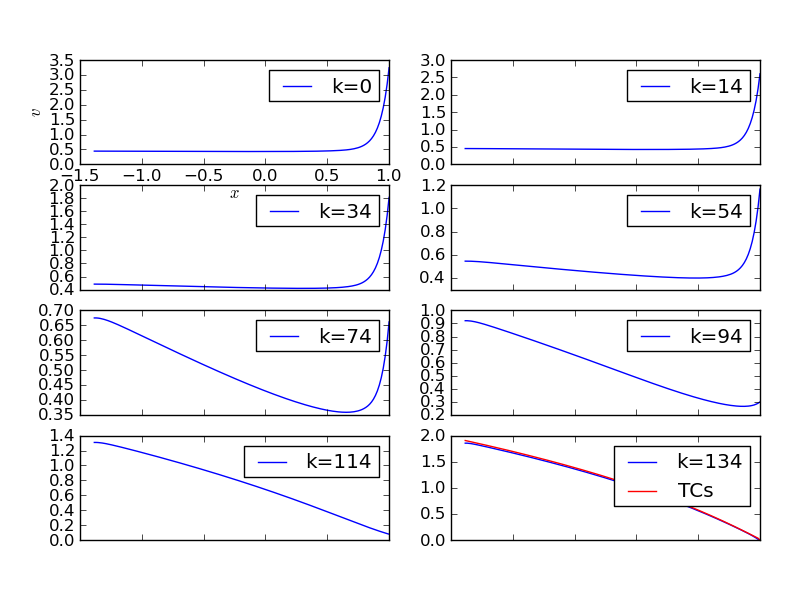
\includegraphics[width=0.48\textwidth]
{Figs/HJB/soln_al=-20_au=20__t=5_b=8.png}
}
\subfloat[Controls, $\a$]
{
\label{fig:HJB_attempt_control}
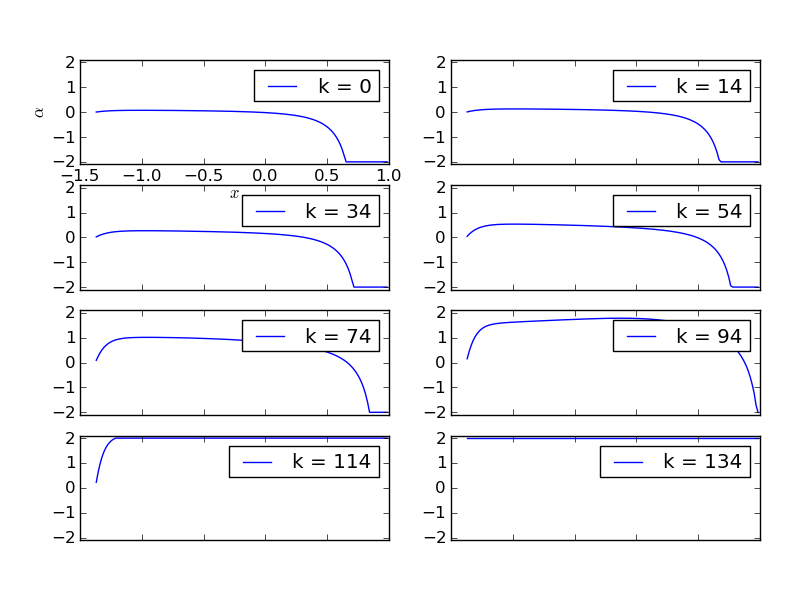
\includegraphics[width=0.48\textwidth]
{Figs/HJB/control_al=-20_au=20__t=5_b=8.png}
}
\caption[]{The solution and controls for the HJB PDE parametrized by:
$\tc = 0.50,  \beta = 0.75,
\amin = -2.00, \amax = 2.00, \eps=0.10,
\T = 1.80$. The $k$ index indicates the time-step, and recall that we are
running backwards in time, so the computation actually happens from right-to-left, bottom-to-top}
\label{fig:HJB_attempt}
\end{center}
\end{figure}

\section{Open-loop Stochastic Control}
As we have mentioned before, when the value of $X_t$ is unknown, one should use
the transition density to perform the optimization. The transition density, $f$,
of $X$, conditional on no spikes having occurred satisfies a Fokker-Planck
equation with absorbing boundaries
\begin{equation}
\begin{gathered}
\di_t f(x,t) =
				\frac{\b^2 }{2}\cdot \di^2_x f -  
				\di_x \Big[ \left(\a(t)- \frac{x}{\tc}\right)  \cdot f \Big]
\\
\\
\begin{array}{lll}
	&\textrm{st.\ }& 
	\left\{ \begin{array}{lcl}
	 f(x,0) &=& \delta(x) \quad \textrm{delta function}
	\\
	(\a(t)- \tfrac x \tc)f - \di_x \tfrac {\b^2}2 f] \big|_{x=\xmin} &\equiv& 0
	\quad \textrm{reflecting BCs at some } \xmin 
	\\
	f(x,t) |_{x=\xth} &\equiv& 0 \quad \textrm{absorbing BCs at } \xth
\end{array} \right. 
\end{array}
\label{eq:FP_pde_OU_PDF}
\end{gathered}
\end{equation}

The $f$ dynamics can also be written as
$$
\di_t f(x,t) = - \di_x \phi(x,t)
$$
for the probability flow, $\phi$, 
$$
\phi(x,t) = (\a- \tfrac x \tc)f - \di_x [\tfrac {\b^2}2 f]
$$
Then the lower BC is
$$
\phi(x,t) |_{x=\xmin} \equiv 0
$$

With this, our objective, \cref{eq:OC_LS_variance}, becomes
$$
J(\a) = \Exp\left[
(\ts - \T \big)^2 
+  
\e \int_0^\ts  \a^2(s) \intd{s}
\right]
$$
Rewriting this in terms of $f$ reads:

\begin{align}
J(\a) =& 
\int_\xmin^\xth \Exp[\t^2|x, \amax] \cdot f(x,\T) \intd{x}
\notag
\\
&+ \int_0^\T \phi(\xth, t) (t-\T)^2 \intd{t}
\notag
\\
&+  \e \int_0^\ts  \a^2(t)  \int_\xmin^\xth f(x,t) \intd{x} \intd{t}
\label{eq:OC_LS_variance_density}
\end{align}

To find the optimal control, $\a = \argmin J[\a]$, the Maximum Principle,
\cite{Ahmed1981} introduces an adjoint variable, $p$,
which solves a PDE related to the PDE satisfied by the density $f$ and then calculates the optimal
control, $\a$ as a function(al) of $f$ and $p$.

In short, the equation for the adjoint, $p$, is 
\begin{equation}
\begin{gathered}
\begin{aligned}
\di_t p =&   
			- \Big[ \frac{\b^2 }{2}\cdot \di^2_x p +  
			(\a(t)- \frac{x}{\tc})  \cdot \di_x p \Big] 
\end{aligned}
\\
\st  
\begin{cases}
	p(x,\T) &= \Ttwo(x)
	\\ 
	\di_x p  \big|_{x=\xmin} &\equiv 0
	\\
	p \big|_{x=\xth} &\equiv (s-T)^2
\end{cases}
\label{eq:adjoint_pde_OU}
\end{gathered}
\end{equation} 

and then $\a$ can be found via
\begin{equation}
\Big\{
 \tilde{\e}  2 \a(t)
+ p f \Big|_\xmin
- \int _\xmin^\xth p \cdot \di_x f \intd{x} 
\Big\} = 0
\quad \forall t \in [0,T]
\label{eq:J_necessary_condition}
\end{equation}

More practically, the quantity, 
$$\di_\a J =  \Big\{
 \tilde{\e}  2 \a(t)
+ p(x,t) f(x,t) \Big|_\xmin
- \int _\xmin^\xth p \cdot \di_x f(x,t) \intd{x} 
\Big\}
$$
gives us the direction of increase of $J$ at $\a(t)$
and we can use it as a gradient in a descent algorithm, given some initial
guess, $\a_0(t)$, for the control.

We show an iteration for finding the optimal control in
\cref{fig:FP_adjoint_objective_control_convergence}.
\begin{figure}[h]
\begin{center}
\subfloat[$\a_k(t)$ ]
{
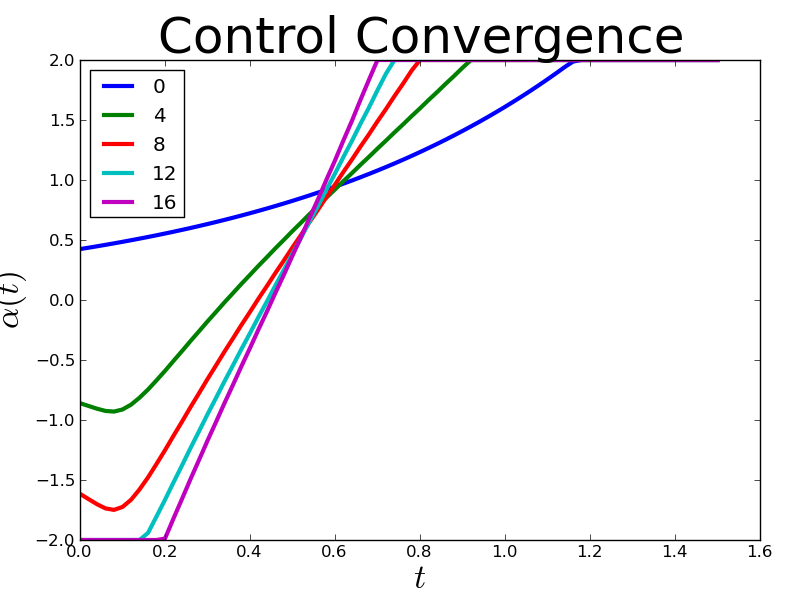
\includegraphics[width=0.48\textwidth]
{Figs/FP_Adjoint/ExampleControlConvergence_control.png}
}
\subfloat[$J_k$ ]
{
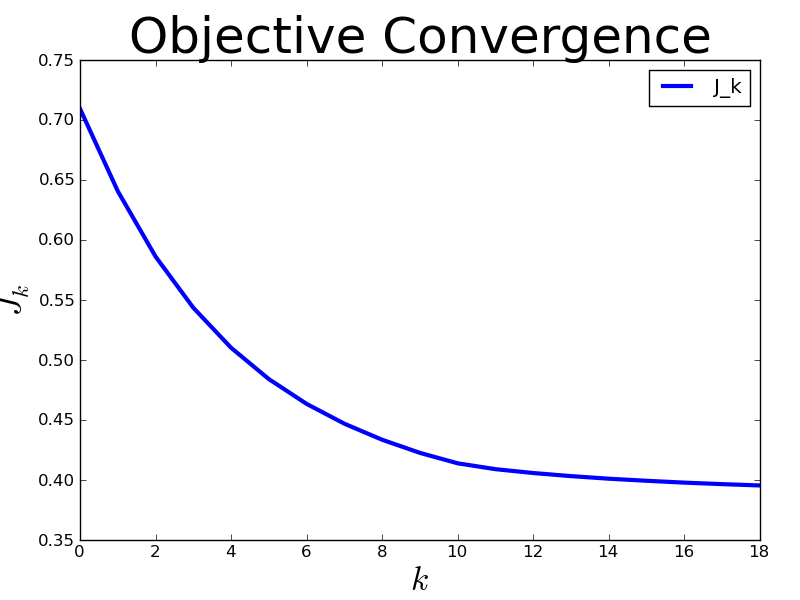
\includegraphics[width=0.48\textwidth]
{Figs/FP_Adjoint/ExampleControlConvergence_objective.png}
}
\caption[ ]{The result of an entire optimization iteration, on the left the
iterates of the control, $\a_k(t)$, on the right the progress of the
objective with each iteration. The final control, in purple, is inhibitory at
the beginning of the time interval, $\a < 0$, unlike the the deterministic
control solution. 
We see a significant
reduction in the objective value, $J$, and thus an improvement, on the
order of 50\%.}
\label{fig:FP_adjoint_objective_control_convergence}
\end{center}
\end{figure}

% \begin{table}[h] 
% \centering
% \begin{tabular}{lc}
% Control Law & Squared Error \\
% \hline
% Deterministic &  0.647 \\
% Stochastic &  0.336\\
% Theory (Value function) & 0.285
% \end{tabular}
% \caption{Realized performance of the different control laws and the theoretical
% expected performance of the stochastic law (last row)}
% \label{tab:realized_avg_errors_det_vs_stoch}
% \end{table}
% 
% \begin{figure}[h]
% \begin{center}
% \subfloat[A]
% {
% \label{fig:controlled_traj_ex1}
% \includegraphics[width=0.33\textwidth]
% {Figs/ControlSimulator/example_controlled_trajectories_id1.png}
% }
% \subfloat[B]
% {
% \label{fig:controlled_traj_ex2}
% \includegraphics[width=0.33\textwidth]
% {Figs/ControlSimulator/example_controlled_trajectories_id4.png}
% }
% \subfloat[C]
% {
% \label{fig:controlled_traj_ex3}
% \includegraphics[width=0.33\textwidth]
% {Figs/ControlSimulator/example_controlled_trajectories_id3.png}
% }
% \caption[]{Examples for the controlled trajectories using both the deterministic
% and the stochastic control approaches. The red vertical line in the plots
% indicates the desired spike-time, $\T$. In A, B the performance of both
% control laws is essentially the same, but in C we see the advantage of the
% stochastic approach. $\tc, \b = [.75, 1.25]$.}
% \label{fig:control_trajectories_examples}
% \end{center}
% \end{figure}
% \begin{figure}[htp]
% \begin{center}
%   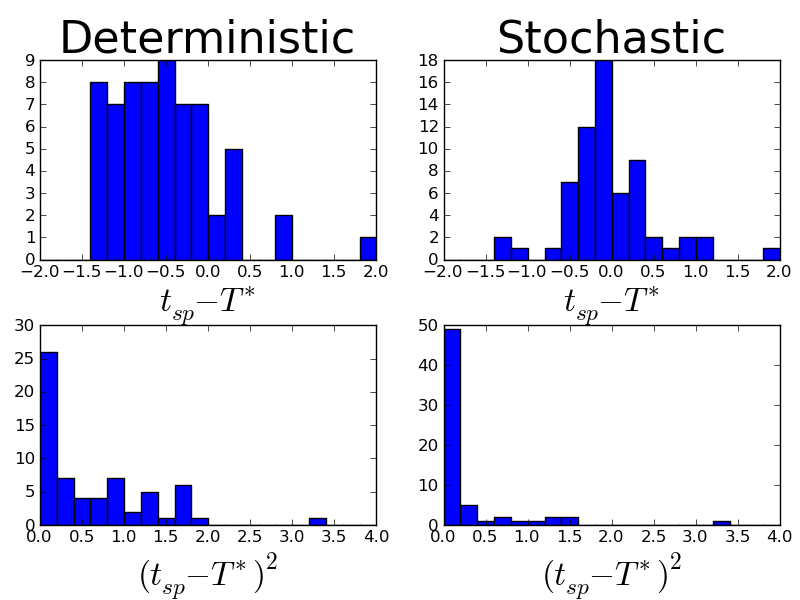
\includegraphics[width=.9\textwidth]{Figs/ControlSimulator/example_controlled_trajectories_hists.png}
%   \caption[labelInTOC]{Histogram of the spike timing error for the
%   deterministic (left) vs. the stochastic (right) control laws.}
%   \label{fig:error_histograms_det_vs_stoch}
% \end{center}
% \end{figure}


\section{Test Comparison of Different Controls}
\label{sec:probabilistic_numerical_test}
We now compare the performance of the optimal closed-loop and open-loop controls
as well as a very naive open-loop controller, which is obtained by assuming
$\b=0$. This naive controller is called 'Deterministic', since it assumes
deterministic dynamics in $X_t$. 

For the comparison we sample $128$ realizations of the controlled system
and apply in turn each of the three controls.

We set $\e = .001$ and $\amax = 2.0$. As such the energy cost is of
secondary importance and the paramount effect on the objective is the difference
$(\ts - \T)$, which we are trying to minimize. We set $\tc, \b = [.75, 1.25]$.

The performance of the three controllers is given in
\cref{tab:realized_avg_errors_det_vs_openloop_vs_stoch} and in
\cref{fig:error_histograms_det_vs_openloop_vs_stoch}.


\begin{table}[h] 
\centering
\begin{tabular}{lcc}
Control Law & Squared Error &  Squared Error \\
 & Empirical & Theoretical\\
\hline
Deterministic &  0.621 & - \\
Open-Loop Stochastic & 0.356 & 0.382\\
Feedback Stochastic &  0.288& 0.285\\
\hline
\end{tabular}
\caption{Realized and theoretical performance of the different control laws. The empirical
performance is obtained using 128 sample paths. The theoretical performance is
found using the $J$ in for the open-loop stochastic control and the value
function $v(x=0, t =0)$ for the closed-loop stochastic control.}
\label{tab:realized_avg_errors_det_vs_openloop_vs_stoch}
\end{table}

\begin{figure}[h]
\begin{center}
\subfloat[]
{
\label{fig:controlled_traj_ex1}
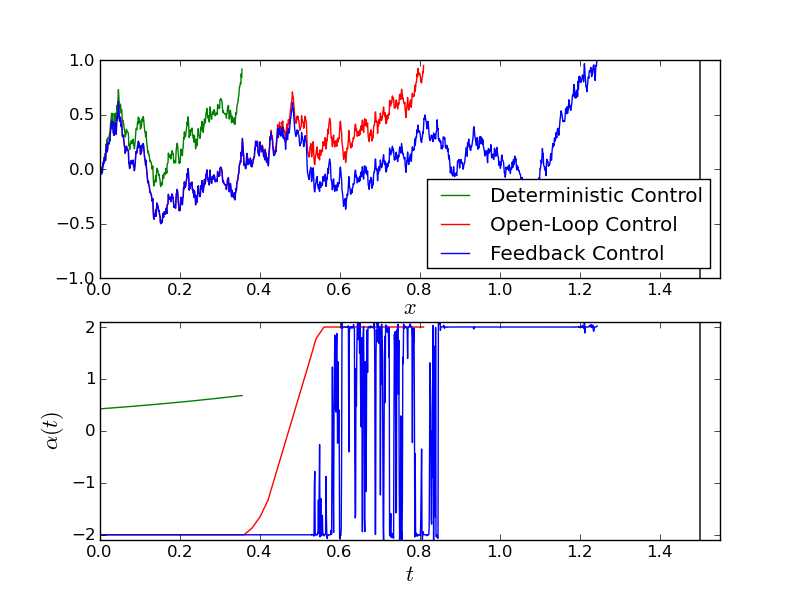
\includegraphics[width=0.33\textwidth]
{Figs/ControlSimulator/3controls_example_trajectories_id3.png}
}
\subfloat[ ]
{
\label{fig:controlled_traj_ex2}
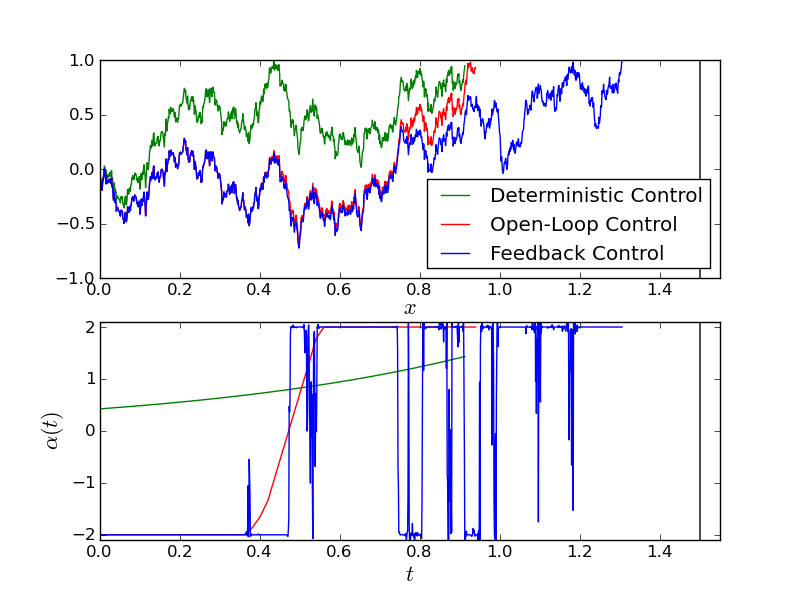
\includegraphics[width=0.33\textwidth]
{Figs/ControlSimulator/3controls_example_trajectories_id5.png}
}
\subfloat[ ]
{
\label{fig:controlled_traj_ex3}
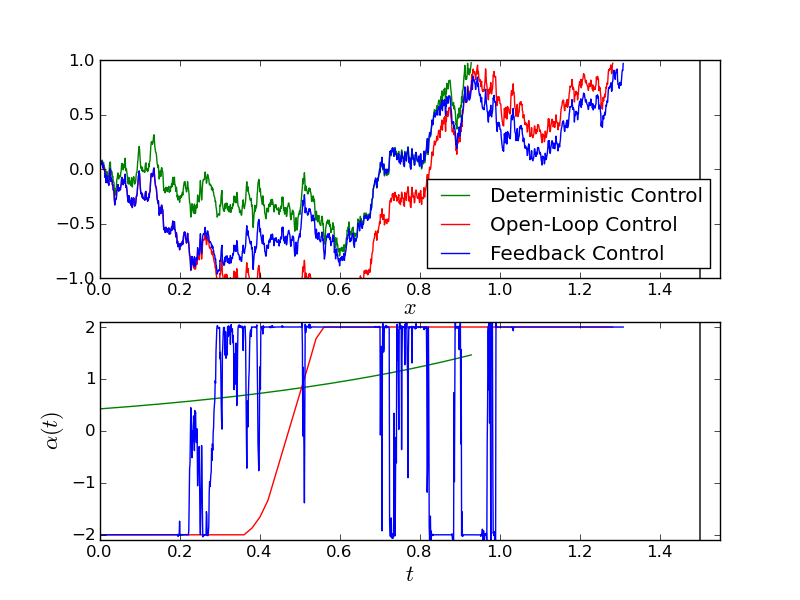
\includegraphics[width=0.33\textwidth]
{Figs/ControlSimulator/3controls_example_trajectories_id6.png}
}
\caption[]{Examples for the controlled trajectories using the deterministic,
open-loop stochastic and feedback stochastic control approaches. The
black vertical line in the plots indicates the desired spike-time, $\T$.
For the parameter values are $\tc, \b = [.75, 1.25]$. The three panels are
three different realizations of the model dynamics.}
\label{fig:control_trajectories_examples}
\end{center}
\end{figure}

\begin{figure}[h]
\begin{center}
  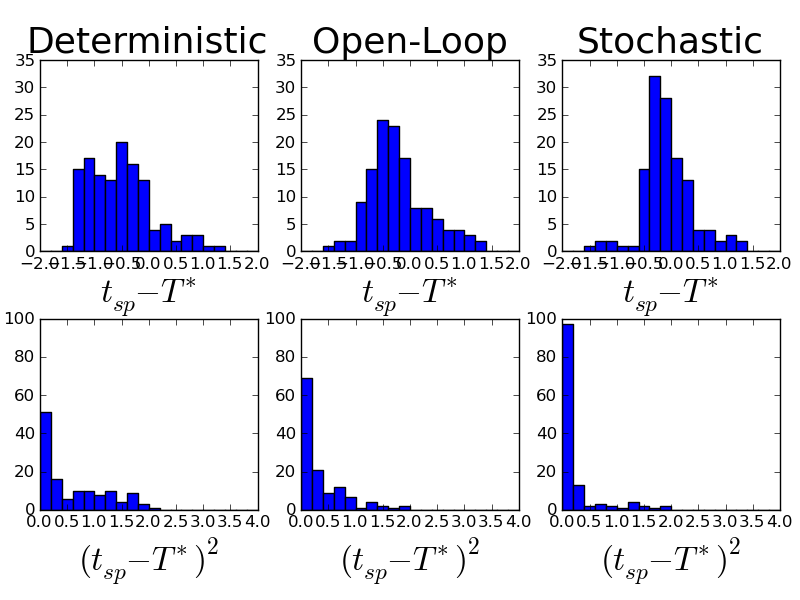
\includegraphics[width=.95\textwidth]
  {Figs/ControlSimulator/3controls_example_trajectories_hists.png}
  \caption[labelInTOC]{Histogram of the spike timing error for the
  deterministic (left) vs. open-loop stochastic(centre) vs. feedback stochastic
  (right) control laws, using the same parameter set as in \cref{fig:control_trajectories_examples}. We have used $N=128$ sample paths
  to form the statistics}
  \label{fig:error_histograms_det_vs_openloop_vs_stoch} 
\end{center}
\end{figure}


\bibliographystyle{plain}
\bibliography{library,local}

\end{document}
